\documentclass[12pt,a4paper]{article}
\usepackage[utf8]{inputenc}
\usepackage{amsmath}
\usepackage{amsfonts}
\usepackage{amssymb}
\usepackage{graphicx}
\usepackage[left=1cm,right=1cm,top=2cm,bottom=2cm]{geometry}
\begin{document}

{\Large Représenter des nuages de points issus d'une expérience}

\bigskip

{\Large 1. Exemple :}

\medskip

\textbf{Fichier de données :}

On dispose d'un fichier "maxpid.txt" donné dans le répertoire d'échange. Il contient deux premières lignes de texte rappelant le nom des grandeurs mesurées et les unités de ces dernières. Les 42 lignes suivantes contiennent 7 nombres correspondant à une date, une consigne, une position, une tension moteur, et d'autres grandeurs mesurées lors d'un essai. 

\medskip
Extrait du fichier de données:

\medskip

\hspace{2cm}\begin{minipage}{0.7\linewidth}
\begin{verbatim}
Temps	Consigne	Position	Commande	Courant	Vit. Axe	Moteur
ms	degrés	degrés	Volts	mA	rad/s	rad/s
    0 	 44.6 	 44.6 	  0.2 	   50 	 0.00 	 -141
    5 	 83.6 	 44.6 	 21.1 	 4650    0.32	  -82
   24 	 83.6 	 45.6 	 21.1 	 3800 	 0.42 	  -33
   44 	 83.6 	 47.9 	 21.1 	 2650 	 0.73 	   -3
   63 	 83.6 	 50.4 	 21.1 	 2100 	 1.02 	   12
   83 	 83.6 	 53.2 	 21.1 	 1700 	 1.44 	   24
  108 	 83.6 	 56.3 	 21.1 	 1500 	 1.57 	   29
  125 	 83.6 	 59.2 	 21.1 	 1400 	 1.84 	   32
\end{verbatim}
\end{minipage}




\medskip

\textbf{On souhaite représenter la colonne position (colonne 2)  en fonction du temps (colonne 0) .
}



\bigskip

\textbf{Traitement du fichier de données:
}
\begin{itemize}
\item Copier et coller le fichier trace\_fich.py dans son répertoire personnel. 
\item Adapter le chemin d'accès au fichier de données dans la méthode np.loadtxt .
\item Exécuter le fichier. Observer. 
\item Observer ce qu'apportent certaines commandes en les dé-commentant.
\end{itemize}

\textbf{Les variables de type array}

Que fait la méthode \textit{loadtxt} de la bibliothèque NumPy? 
exemple : 

$X=np.loadtxt("I:/Jacques/LK_2015/IPT/maxpid.txt",skiprows=2)$

\medskip


A tester dans le shell Python:
\begin{enumerate}
\item Quel est le type de X ?
\item Que contient X[5]?
\item Que contient X[5,0]?
\item Que contient X[:,0]
\item Que donne la commande X.shape ?
\end{enumerate}

Pour être plus direct on aurait pu utiliser des options dans la commande:

\begin{verbatim} t,position= 
loadtxt("I:/Jacques/LK_2015/IPT/maxpid.txt",usecols=(0,2),skiprows=2,unpack=True) 
\end{verbatim}

L'option unpack=True a permis de créer 2 tableaux  t et position à partir des colonnes t et position.

\newpage

\textbf{Image obtenue dans l'exemple :}

\begin{center}
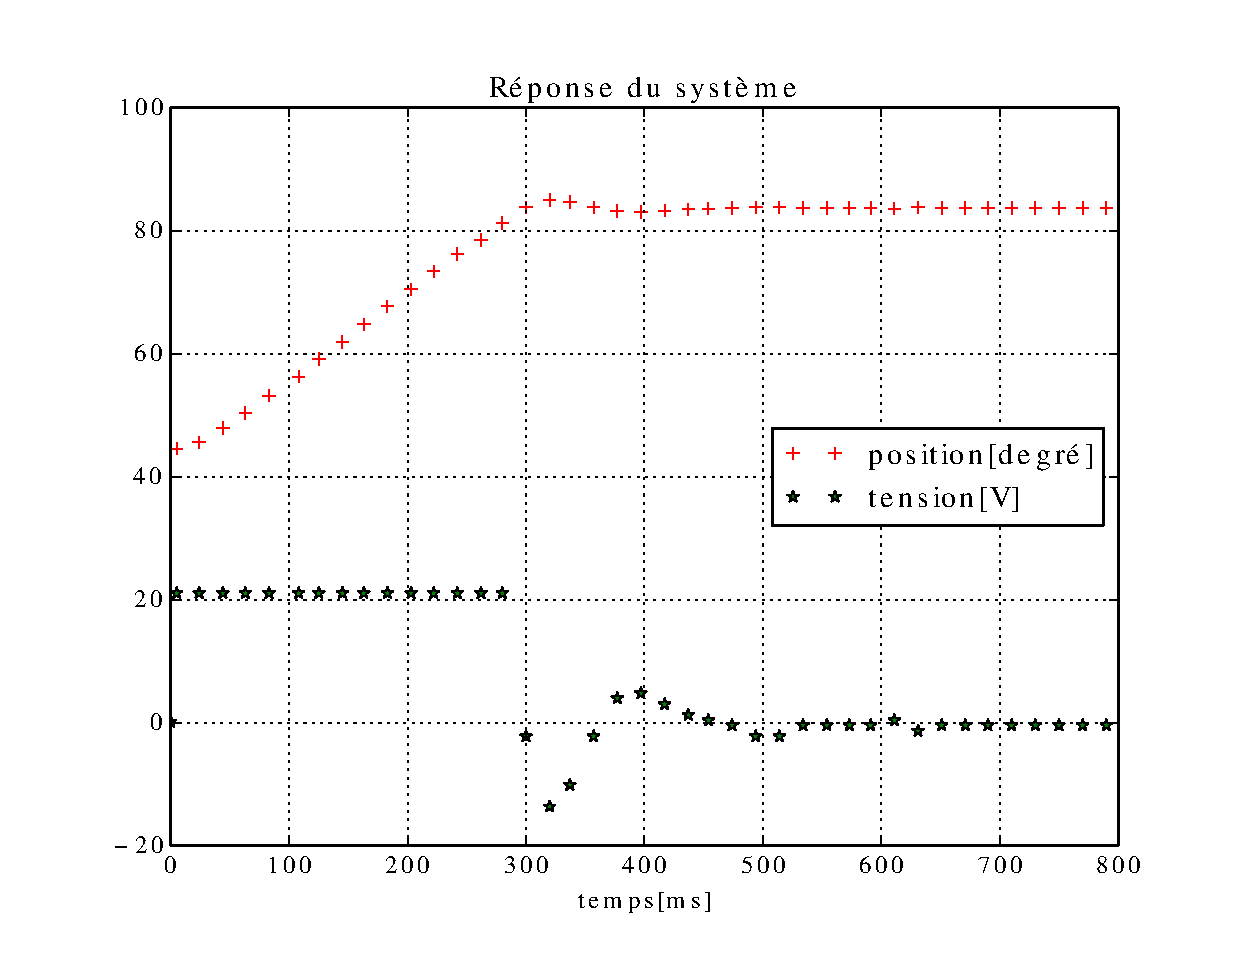
\includegraphics[scale=1]{../../../LK_2015/IPT/figure1.eps} 
\end{center}

{\Large 2. Exercice }:

Dans le fichier de données \textbf{moto.txt}, la colonne 2 représente la mesure en Volt d'une accélération, le temps est absent du fichier, mais on sait qu'entre deux lignes s'est écoulé 0,002s. On souhaite représenter l'accélération en fonction du temps.

Tester dans le shell Python la commande np.arange(0,2,0.1); s'en inspirer pour créer la tableau du temps.

Tester dans le shell Python la commande np.linspace(0,2,21); s'en inspirer pour créer la tableau du temps.
\end{document}
